\chapter{Heterogenous Production Functions, Panel Data, and Productivity Dispersion}
\begin{center}
\large
\textsc{Jeremy Fox, Vitor Hadad, Stefan Hoderlein} \\ \textsc{Amil Petrin, Robert Sherman}
\end{center}

\doublespacing

\section{Introduction}

% [One or two sentences providing basic introduction to the field, comprehensible to any economist]
Econometricians often need control for unobserved heterogeneity, 

%[Two to three sentences of a more detailed background, comprehensible to econometricians]

%[One sentence clearly stating the general problem being addressed by this particular study]
In the context of panel data, it has become standard to controlling for unobserved heterogeneity via a \emph{fixed effects} approach, where we do not impose restrictions the distribution of latent heterogeneity parameters conditional on observable characteristics \citet{wooldridge2010econometric}. However, this flexibility often comes at a cost in terms of statistical modeling: the most ubiquitous fixed effects strategy in panel data is via the introduction of a time-invariant random intercept.[\ref{}, \ref{}, \ref{}], but there are many instances of economic problems where this is might not be appropriate (e.g. [QUICK EXAMPLE]).

%[One sentence summarizing main result]
Here, we present constructive identification and estimation results for the moments and marginal distribution of random coefficients in a linear panel data model with \emph{two} random coefficients
\begin{align}
  Y_{it} = A_{it} + X_{it}B_{it} + Z_{it}^{T}\beta_{t}
\end{align}

\noindent where the intercept $A_{it}$ and slope $B_{it}$ follow a specific autoregressive process but are otherwise allowed to be arbitrarily correlated with all regressors, and $Z_{it}$ is a (potentially large) vector of covariates associated with individual-invariant coefficients $\beta$.


% [Two or three sentences explaining what the main results reveals in direct comparison to what was thought to be case previously, or how the main result adds to previous knowledge]
% [One sentence to put the results into more general context]
Our results develop upon and extend the results of earlier work by \cite{graham2012identification}, who only focus on the first moments of the random coefficients and have stricter timing assumptions than ours. Another paper is \cite{arellano2011identifying}, who, like us, provide a method for identification and estimation of higher moments and distributional characteristics of random coefficients, but they maintain certain regularity assumptions that we do not impose.  Our model also permits that lagged dependent variables to be regressors. More broadly, this paper contributes to the larger literature of panel data models with unobserved heterogeneity, as we discuss below.


% [Two to three sentences to provide a broader perspective, readily comprehensible to a scientist in any discipline..]
In our particular application, we take $Y_{it}$ to be value-added log-production, while the two random coefficients represent total factor productivity (TFP) and the elasticity of one of the inputs in a Cobb-Douglas model of production. There is strong evidence for heterogeneity in this setting, where it is known as \emph{productivity dispersion}. In the United States, \cite{syverson2004product} finds large plant-level discrepancies in TFP, noting that within four-digit SIC industries ``the plant at the 90th percentile of the productivity distribution makes almost twice as much output with the same measured inputs as the 10th percentile plant", and a later survey by \cite{syverson2011determines} confirms this to be a typical finding. In fact, other work by \citep{hsieh2009misallocation} indicates that this gap may be small compared to other countries. In our work we note, however, that the large observed variation in TFP might be a product of restrictive statistical models: when only the intercept is able to vary, it may end up absorbing most the heterogeneity in the data, leading to inflated estimates of the standard deviation. On the other hand, we remark that our specific model and data differ from the ones above so we cannot directly comparison our results, but leave it as a suggestion for future research.



% ----------------------
% LITERATURE REVIEW 
% ----------------------

\section{Literature review}

In full generality, panel data models can be represented as
\begin{align}
  Y_{it} = m(H_{it}, X_{it}, U_{it}) \label{eq:full_generality_panel}
\end{align}

\noindent where $Y_{it}$ is the dependent variable of interest for unit $i$ at period $t$, $H_{it}$ is an individual-specific, possibly infinite-dimensional object often called the \emph{unobserved heterogeneity} component, $X_{it}$ are observable characteristics, and $U_{it}$ is an idiosyncratic error term. For example, $Y_{it}$ might represent an individual's wages over time, $X_{it}$ a vector of characteristics that includes educational attainment, $H_{it}$ a measure of their cognitive or manual ability, and $U_{it}$ measurement error. The econometrician is usually interested in some functional of this object, such as the causal average effect of on $Y_{t}$ of a change in $X_{it}$ (known as the \emph{average partial effect} of education on wages). 

Particular care must be taken with the \emph{unobserved heterogeneity} parameter $H_{it}$. \citet[~p.2]{browning2007heterogeneity} define \emph{heterogeneity} as ``the dispersion in factors that are relevant and known to individual agents when making a particular decision"\footnote{Browning \textit{et al} were, in turn, paraphrasing \cite{cunha2005separating}}. The qualifier \emph{unobserved} serves to emphasize that the econometrician does not have access to information about such factors. This is problematic because, even when $H_{it}$ itself is not of interest, it may preclude the identification of causal objects To continue our running example: even if we observe that workers with higher educational attainment receive higher wages, we cannot a priori claim that we have found a causal effect of $X_{it}$, as it may be that high-ability ($H_{it}$) workers are able to self-select into higher-paying jobs.

One of the foremost advantages of dealing with panel data is that, under specific assumptions, we are able to control for the unobserved heterogeneity component. However, without further assumptions, however, nothing can be said. Therefore, econometricians have posited a number of restrictions on the model above, each producing different identification strategies.

Econometric applications (such as \cite{???}, \cite{???} often to cite a few) assume that $m$ is a linear function.
\begin{align}
  Y_{it} = A_{it} + X_{it}^{T}B_{it} + U_{it}
\end{align}

\noindent where $H_{it} = [A_{it}, B_{it}]$, a vector of \emph{random coefficients}. Furthermore, they will often impose additionally that 
\begin{align}
  Y_{it} = A_{i} + X_{it}^{T}\beta + U_{it}
\end{align}

and that unobserved heterogeneity appears only as an intercept.

% One of the main objectives is to model heterogeneity


% Importance of controlling for heterogeneity

Imposing different restrictions will give rise to different identification strategies. As recounted by \cite{graham2012identification}, the \emph{fixed effects} method implies restrictions on the functional form $m$ and on the conditional distribution of the idiosyncratic shocks $F(U_{it}|X_{\cdot}, A_{\cdot})$, but leaves the conditional distribution of unobserved heterogeneity $F(A|X)$ unrestricted. A related method, named \emph{random effects}, entails imposing an independence assumption between $A_{\cdot}$ and $X_{\cdot}$, but that usually leads to models that are harder to motivate economically.



Further restrictions can be imposed for simplicity.

Figure \ref{fig:panel_data_models} illustrates the difference between them.

[[[These APEs are essentially derivatives of the average structural function of Blundell and Powell (2004).]]]


In this paper we focus on the more general case where we allow for more than one random coefficient, and also allow them to be correlated with the regressor. The literature dealing with this more general case is substantially smaller. \citet{hoderlein2010analyzing} analyzed a for any number of random coefficients, but required the stronger assumption that the coefficients are independent from the regressors. 

% Closest works are Chamberlain (1982), Arellano and Bonhomme (2011), Graham nd Powell (2012), Evdokimov (2011)]


% Production function estimation
> Recent papers on heterogeneous production functions Kasahara, Shrimpf and Suzuki (2016), Balat, Brambilla and Sazaki (2016)
  Extend proxy variable approaches but require variables to be chosen in period t − 1 with only static considerations, as in FOCs. Ackerberg and Hahn (2016)
  Scalar unobservable enters into nonparametric production function


  \begin{figure}
    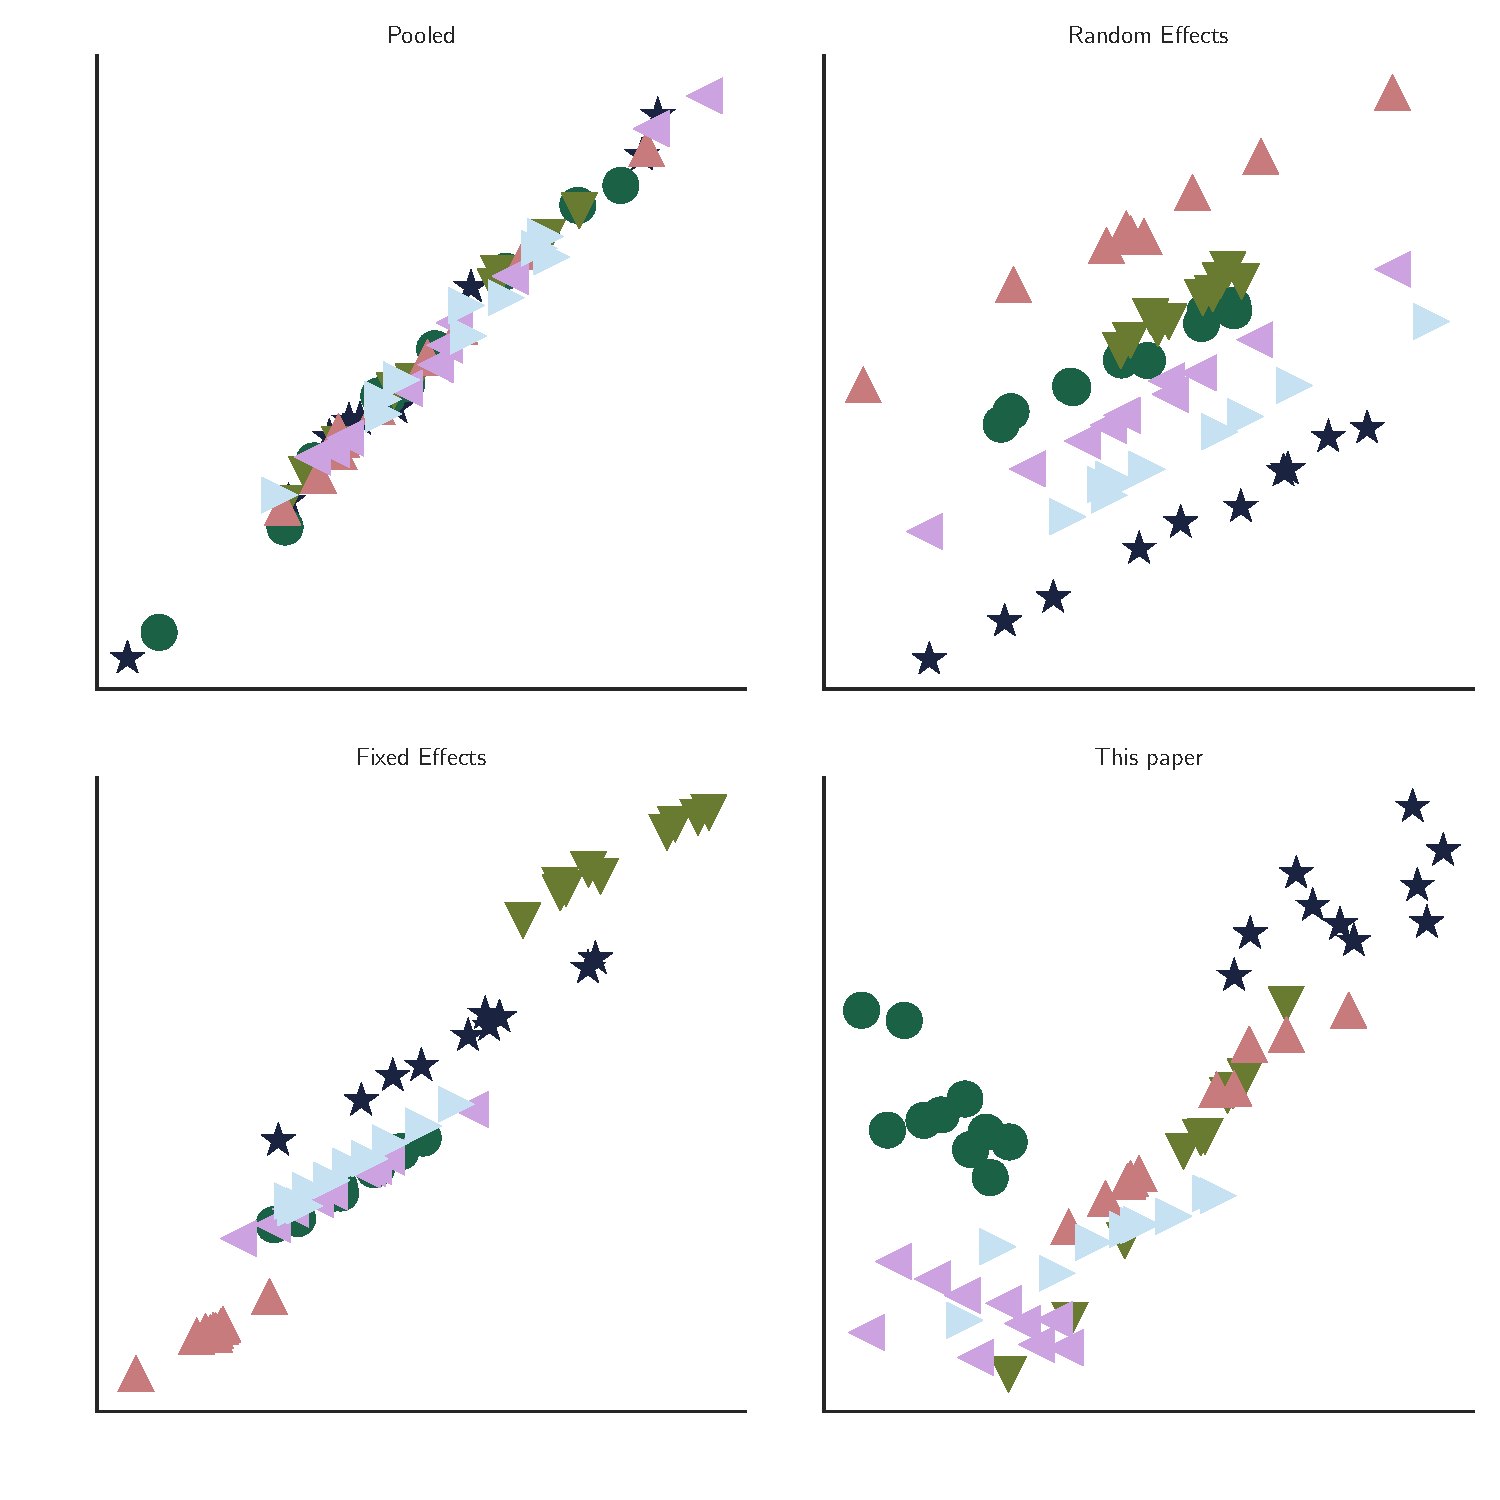
\includegraphics[width=1\textwidth]{/Users/vitorhadad/Documents/kidney/matching/phd_thesis/chapter1/figures/panel_data_models.pdf}
    \caption[Linear panel data models]{\textbf{Linear panel data models} \\ Different assumptions leading to different panel data models. Each different marker type and color indicates a different individual. \emph{Pooled}: all observations share same intercept and slope; \emph{Random effects}: each observation possesses their own time-invariant slope, but all share the same slope; \emph{Fixed effects}: same as random effects, but intercept and regressors can be correlated (figure shows positive correlation); \emph{FHHPS}: our paper generalizes the model by 1) allowing for intercept and slope to be correlated with regressors, and 2) allowing both intercept and slope to drift according to a specific Markovian process.}
    \label{fig:panel_data_models}
  \end{figure}


\section{Model and assumptions}

In order to reduce clutter we will drop the $i$ subscript. For $1 \leq t \leq T$, define
\begin{align*}
Y_{t} &= A_{t} + B_{t}X_{t}
\end{align*}
where $X_{t}$ is a scalar, and $A_{t}, B_{t}$ are scalar random coefficients that evolve according to an AR(1) Markov process.
\begin{align}
  A_{t} &= A_{t-1} + U_{t} \\
  B_{t} &= B_{t-1} + V_{t}  
\end{align}

We will make the following sufficient assumptions for identifiability. Some of these are known to be stronger than necessary, and we will mention how to relax them later on. For ease of notation, let us denote $W_t = [X_t, X_{t-1}]^{T}$

\begin{assumption}{} \label{a:timeindependence}
  Conditional on recent covariates $W_t$, contemporaneous shocks are independent from past shocks.
  \begin{align}
    \text{For }2 \leq t \leq T ,
    \quad     
    (U_t, V_t) \perp \{ U_s, V_s \}_{s=0}^{t-1} \  | \ W_t
  \end{align}
\end{assumption}


\begin{assumption}{} \label{a:sequentialindependence}
  Shocks are sequentially independent from all covariates
  \begin{align}
    \forall t, \qquad U_t, V_t \perp (X_{1}, \cdots, X_{T})
  \end{align}
\end{assumption}


\begin{assumption}{}  \label{a:support}
  The covariate associated with the random coefficient is continuously distributed and is supported on the entire real line for all periods. Furthermore, their joint distribution is non-degenerate.
  \begin{align}
    \text{supp}(X_1) = \cdots = \text{supp}(X_T) = \mathbb{R} \qquad \text{and} \qquad \forall s \neq t, \ \ P(X_s = X_t) = 0 
  \end{align}
\end{assumption}

\begin{assumption}{}  \label{a:fullrank}
  Nonsingularity of the covariate matrix.
  \begin{align}
    \text{For }2 \leq t \leq T ,
    \quad     
    E[W_tW_t^{T}] \text{is nonsingular}
  \end{align}
\end{assumption}


We should note that assumptions \ref{a:timeindependence} and \ref{a:sequentialindependence} allow for future regressors to be correlated with past shocks. In the context of firm profit maximization, this means that a firm is allowed to choose future inputs based on their previous productivity. In a different context, they would also allow for a dynamic model with $X_t = Y_{t-1}$. Crucially, we have not made any assumptions about contemporaneous independence between random coefficients and regressors, thus allowing for a unobserved heterogeneity of a general type.

Assumption \ref{a:support} is a simplifying ``no-stayer" assumption that will facilitate some of the asymptotic derivations below. Assumption \ref{a:fullrank} is a common technical assumption often used for generic identification in linear models.

\section{Identifying random coefficient moments}

In this section, we show how to identify the $r^{th}$ moments of the random coefficients $(A_{t}, B_{t})$. Broadly, our identification strategy will follow the next steps.

\begin{enumerate}
  \item Identify shock moments $E[U_{t}^{\ell}V_{t}^{r-\ell}]$ 
  
  \item Express the conditional moments of the regressand $E[Y_{1}^\ell Y_{2}^{r - \ell} | W_{2i}]$ as a function of conditional moments of random coefficients $E[A_{t}^{\ell}B_{t}^{r-\ell}|W_{2}]$ and shocks $E[U_{t}^{\ell}V_{t}^{r-\ell}]$ 
  
  \item Invert the above so as to represent conditional moments of random coefficients as a function of conditional moments of the regressand and shocks $E[U_{t}^{\ell}V_{t}^{r-\ell}|W_{2}]$ 
  
  \item Integrate out to get unconditional moments $E[A_{t}^{\ell}B_{t}^{r-\ell}]$
\end{enumerate}

\subsection{First period moments}

Let us start with the first moment ($r = 1$). In this case, we are required to have $T \geq 2$ consecutive waves of panel data. 


We begin by simply reminding ourselves of the system of equations for these two periods.
\begin{align}
  \begin{cases}
    Y_{1} = A_{1} + B_{1}X_{1} \\ 
    Y_{2} = A_{2} + B_{2}X_{2} 
  \end{cases}
\end{align}

Let's expand the coefficients according to our model equations \ref{}.
\begin{align}
  \begin{cases}
    Y_{1} = A_{1} + B_{1}X_{1} \\ 
    Y_{2} = A_{1} + U_{2} + B_{1}X_{2} + V_{2}X_{t} \label{eq:expanded}
  \end{cases}
\end{align}


\paragraph{Step 1} In order to identify shocks, we consider the expectation of the difference between the two periods, conditioning on some point $W_2 = w_2 = (x, x)$.
\begin{align}
  E[Y_{2} - Y_{1} \ | \  W_{2} = w_{2}] = 
  E[U_{2}] + E[V_{2}]x
\end{align}

\noindent The expression above contains two caveats. First, that thanks our full support assumption \ref{a:support}, we can choose any point on $\mathbb{R}^2$ to condition on, including a point where $X_1 = X_2 = x$ as we just did. Second, that Assumption \ref{a:timeindependence} allowed us to drop the conditioning for the shocks.

Now, note that the moments $E[U_2]$ and $E[V_2]$ on the right-hand side are solutions to this minimization problem
\begin{align}
  \min_{\theta_u, \theta_v}  
  E[(Y_{2} - Y_{1} - \theta_u -  x\theta_v)^2 \  | \ W_2 = w_2]
\end{align}
\noindent and that the solution is unique, by virtue of the strict convexity of the quadratic function and the full rank assumption \ref{a:full_rank}. It follows that the shock moments $E[U_2]$ and $E[V_2]$ are generically identified, and so are $\beta_1$ and $\beta_2$.


\paragraph{Step 2} For this step, we simply have to take expectations of \ref{eq:expanded}, now conditioning on $W_2 = w_2 = (x_1, x_2)$. (Note we have dropped the constraint $X_1 = X_2$).
\begin{align}
  \begin{cases}
      E[Y_{1}|W_{2}]
        = E[A_{1}|W_{2}] + E[B_{1}|W_{2}]x_{1} \\ 
      E[Y_{2}|W_{2}]
        = E[A_{1}|W_{2}] + E[U_{2}] + E[B_{1} \ | \ W_{2}]x_{2} + E[V_{2}]x_{2} 
  \end{cases}
\end{align}

\paragraph{Step 3} Writing the previous equation in matrices after a little rearranging, we get:
\begin{align}
  \begin{bmatrix}
    E[Y_{1}|W_{2}] \\  
    E[Y_{2}|W_{2}] - E[U_{2}] -  E[V_{2}]x_{t} 
  \end{bmatrix}
  =
  \begin{bmatrix}
    1 & x_1 \\
    1 & x_2  
  \end{bmatrix}
  \begin{bmatrix}
    E[A_{1}|W_{2}] \\
    E[B_{1}|W_{2}]
  \end{bmatrix}
\end{align}

\noindent As long as $x_1 \neq x_2$, we can invert the first matrix on the right-hand side. 
\begin{align}
  \begin{bmatrix}
    E[A_{1}|W_{2}] \\
    E[B_{1}|W_{2}]
  \end{bmatrix}
  =
  \begin{bmatrix}
    1 & x_1 \\
    1 & x_2  
  \end{bmatrix}^{-1}
  \begin{bmatrix}
    E[Y_{1}|W_{2}] \\  
    E[Y_{2}|W_{2}] - E[U_{2}] -  E[V_{2}]x_{2}  \label{eq:inversion}
  \end{bmatrix}
\end{align}

\noindent since all the quantities on the right-hand side are known, we have identified all the conditional first moment of our random coefficients outside the line $X_1 = X_2$. Since our ``no-stayer" assumption \ref{a:support} guarantees that a randomly drawn point from the joint distribution of $X_1$ and $X_2$ will not be on the diagonal, we have generic identification.

Conditional second-period moments are also automatically identified, since due to our \ref{a:sequentialindependence} assumption we have that shocks are mean-independent from contemporaneous regressors, which allows us to write
\begin{align}
  E[A_2 | W_2 = w_2] = E[A_1|W_2 = w_2] + E[U_2] \\
  E[B_2 | W_2 = w_2] = E[B_1|W_2 = w_2] + E[V_2] \\
\end{align}

\paragraph{Step 4} The final step is simply to integrate out over the distribution of $W_2$ to get unconditional moments. 

\subsection{Second period moments} The identification procedure is analogous, but this time we use the square of our model equations.

\paragraph{Step 1} Identify shock second moments on the diagonal $W_2 = w_2 = (x, x)$ using the following equation
\begin{align}
  E[(Y_{2} - Y_{1})^2 \ | \  W_{2} = w_{2}] = 
  E[U_{2}^2] + E[V_{2}^2]x^2 + 2E[U_{2}V_{2}]x
\end{align}

\noindent The analogous minimization procedure is
\begin{align}
E[U_2^2], E[V_2^2], E[U_2V_2] =
  \min_{\theta_{uu}, \theta_{vv}, \theta_{uv}}  
  E[(Y_{2} - Y_{1} - \theta_{uu} -  x^2\theta_{vv} - 2x\theta_{uv})^2 \  | \ W_2 = w_2]
\end{align}

\noindent point identification is once more possible because the solution to this minimization problem is unique.

\paragraph{Steps 2-3} Again drop the constraint $X_1 = X_2$, and conditioning on $W_2 = w_2 = (x_1, x_2)$ consider the expectation of the square of our model equations.

\begin{align}
\begin{bmatrix}
  E[A_1^2 | x_{1}, x_{2}] \\ 
  E[B_1^2 | x_{1}, x_{2}]  \\ 
  E[A_1 B_1 | x_{1}, x_{2}]
\end{bmatrix}
=
\begin{bmatrix}
  1 & x_{1}^2 & 2x_{1} \\ 
  1 & x_{2}^2 & 2x_{2} \\ 
  1 & x_{1}x_{2} & x_{1} + x_{2} \\ 
\end{bmatrix}^{-1}
\begin{bmatrix}
  E[Y_1^2 | x_{1}, x_{2}] \\
  E[Y_2^2 | x_{1}, x_{2}] - C_{1i} \\
  E[Y_1 Y_2 | x_{1}, x_{2}] - C_{2i} \\
\end{bmatrix}
\end{align}

\noindent where $C_{1i}$ and $C_{2i}$ involve only quantities that were already estimated in previous steps.
\begin{align}
C_{1i} &= E[U^2] + 2E[U_2 V_2] x_{2} +  E[V_2^2]x_{2}^2 \\
      &- 2\{
E[A_1 | x_{1}, x_{2}] +
E[B_1 | x_{1}, x_{2}]x_{2}
\}
\{
E[U_2] + E[V_2]x_{2}
\}
\\
C_{2i} &= 
\{ 
  E[A_1 | x_{1}, x_{2}] + E[B_1 | x_{1}, x_{2}]x_{1}
\}
\{
E[U_2] + E[V_2]x_{2}
\}
\end{align}

Note that the relevant matrix above is invertible whenever $x_1 \neq x_2$. 

\paragraph{Step 4} Analogous to step 4 in the first moment case.


\subsection{Identifying further moments}

The argument above generalizes for arbitrary moments. In fact, if we are only after moments a finite number of moments of the distribution, then assumption \ref{a:sequentialindependence} as follows. Let $r$ be a positive integer and for $t \geq 2$ define $W_t = (X_{t-1}, X_{t})$. We will say that $(U_t, V_t)$ are \emph{r\textsuperscript{th}-moment independent} of $W_t$ if 
  \begin{align}
    \text{For }1 \leq j \leq r,
    \quad     
    E[U_{t}^{r-j} V_{t}^{j} | W_t] = E[U_{t}^{r-j} V_{t}^{j}]
  \end{align}
\end{definition}

We can replace assumption \ref{a:sequentialindependence} by the following weaker assumption.

\paragraph{Assumption 3.1'} \label{a:sequentialindependence}
  \textot{Shocks are r\textsuperscript{th}-moment independent from all covariates}
  \begin{align}
    \text{For }1 \leq j \leq r,
    \quad     
    E[U_{t}^{r-j} V_{t}^{j} | W_t] = E[U_{t}^{r-j} V_{t}^{j}]
  \end{align}
  
  

\subsection{Extension: fixed coefficients}

Our model can be augmented with an arbitrary number of regressors associated with coefficients that are individual-invariant -- but not necessarily time-invariant. The model equations become
\begin{align*}
Y_{t} &= A_{t} + B_{t}X_{t} + Z_{t}^T \beta_{t} \qquad \beta_{t}: \text{fixed}
\end{align*}

Identification of the fixed coefficients happens on Step 1, when the minimization problem becomes
\begin{align}
 E[U_2], E[V_2], \beta_1, \beta_2  = \min_{\theta_u, \theta_v, \theta_{b_1}, \theta_{b_2}}  
  E[(Y_{2} - Y_{1} - a - bx_2 + z_2^{T}\theta_{b_1} - z_1^{T}\theta_{b_2})^2 | W_2 = w_2]
\end{align}
and the argument follows for the same reasons that were previously explained. Once we have identified $\beta_1, \beta_2$, we remove them from future computations using the modified regressand $\tilde{Y_t} := Y_{t} - Z_{t}\beta_{t}$, and the rest of the process delineated above goes through without further change.



\subsection{Identifying the marginal distribution of random coefficients}

In this section we will prove that we can identify the marginal density of random coefficients $f_{A_tB_t}$. We begin by strengthening the 


%--------------
% ESTIMATION
%------------- 


\section{Estimation} \label{sec:estimation}

Our estimation procedure follows three steps:

\begin{enumerate}
  \item Use local polynomial regression to estimate shock moments and individual-invariant coefficients
  \item Use any nonparametric estimator to retrieve estimates of random coefficient moments conditional on observables
  \item Average out conditional random moments by averaging out conditional moments, taking care to avoid
  observations for which $X_1 \approx X_2$.
\end{enumerate}

Let us consider each one of these steps in detail.

\subsection*{Estimating shocks}

\paragraph{First moments} Regress $\Delta Y_2$ on $X_2$ locally at the diagonal $X_1 \approx X_2$:
\begin{align}
  \hspace*{-1cm}
  (\widehat{E}[U_2], \widehat{E}[V_2], \ \cdot \ ) = \arg \min_{\theta_{U} ,\theta_{V}, \gamma}
\sum_{i} K_h (\Delta X_{2i}) \cdot 
      \left( \Delta Y_{2i} - \theta_{U} - X_{2i}\theta_{V} - g_1(X_{2i}, \Delta X_{2i}; \gamma \right)^2
\end{align}

\noindent where $K_h(\cdot)$ is a standard kernel with asymptotically zero bandwidth:
\begin{align}
  h_{shocks}(n) = c_{shocks}n^{−\alpha_{shocks}} \qquad \text{where } \lim_{n\rightarrow \infty} h_{n} = 0
\end{align}
\noindent and $g_1$ is a $K$-order polynomial in $X_2$ and $\Delta X_2$ with coefficients $\gamma$. In theory its inclusion is optional, but we have observed that its presence substantially improves the quality of the estimates. 

If our model included time-invariant coefficients, they would also be estimated in this step.



\paragraph{Second moments} We estimate the uncentered moments by proceeding similarly to above:
\begin{align}
  (\widehat{E}[U_2^2], \widehat{E}[U_2 V_2] &\widehat{E}[V_2^2], \ \cdot \ ) = \\  
  \arg \min_{\theta_{U_2} , \theta_{UV}, \theta_{V_2}, \gamma}
\sum_{i} K_h(\Delta X_{2i}) &\cdot 
      \left( \Delta Y_{2i}^2 - \theta_{U_2} - 2X_{2i}\theta_{UV}  - X_{2i}^2\theta_{V_2} - g_2(X_{2i}, \Delta X_{2i}; \gamma) \right)^2
\end{align}

Naturally, once we have uncentered second moments and first moments, we can compute estimates of centered moments using the usual formulas for centered moments, e.g. $\widehat{Var}[U_2] = \widehat{E}[U_2^2] - \widehat{E}[U_2]^2$. 

\subsection*{Conditional random coefficient moments}



\paragraph{Conditional moments of $Y_1$ and $Y_2$} Here we begin by estimating $E[Y_1^{m} Y_2^{n}|X_1 = x_1, X_2 = x_2]$ for $m,n \in \{ (1,0), (0,1), (1,1), (2,0), (0,2)\}$. This can be done using any nonparametric estimator, but we choose the Nadaraya-Watson for simplicity.
\begin{align}
  \widehat{E}[Y_1|X_1 = X_1, X_2 = X_2] =
  \frac{\sum_i Y_{1i}K_h(X_{1i} - x_1) K_h(X_{2i} - x_2)}
  {\sum_i K_h(X_{1i} - x_1) K_h(X_{2i} - x_2)}
\end{align}

\noindent where $K_h$ is again a standard kernel endowed with asymptotically vanishing bandwidth.
\begin{align}
  h_{nw}(n) = c_{nw}\hat{\sigma} n^{-\alpha_{nw}}
\end{align}

\noindent where $\hat{\sigma}$ is an estimate of $Std(X_1) = Std(X_2)$. Note that for the theoretical MISE-minimizing bandwidth, one should set $\alpha_{nw} = \frac{1}{6}$. 

\paragraph{Solving for first moments} Once in possession of all the previous estimates, we can solve for estimates of conditional random coefficient moments using the empirical analogs of equations \ref{eq:first_moment_inversion} and \ref{eq:second_moment_inversion}.
  

\subsection*{Unconditional random coefficient moments}

In this final step, we must exclude observations near the diagonal $X_1 ≈ X_2$, and then average the conditional moments associated with the remaining observations. According to our asymptotic results, included observations must satisfy the following conditions:
\begin{align}
  |\Delta X_{2i}| &> c_{cens1} \hat{\sigma}_{X_2} n^{-\alpha_{cens1}} \quad \text{ for first moments}\\
  |\Delta X_{2i}| &> c_{cens1} \hat{\sigma}_{X_2} n^{-\alpha_{cens2}} \quad \text{ for second moments}
\end{align}
  
As shown in section \ref{\asymptotic_results}, the optimal thresholds can be shown to be associated with exponents $\alpha_{cens1} = \frac{1}{4}$ and $\alpha_{cens2} = \frac{1}{8}$. However, theory gives us no guidance regarding the choice of constants $c_{cens1}$ and $c_{cens2}$, so we resort to experimentation in the next section.




% -------------
%  Simulations
% -------------


\section{Simulations} \label{sec:simulation}

The purpose of this sections is to provide a simulation study in a setting that is similar to our empirical application. We begin by generating the first period random coefficients $(A_1, B_1)$, their second-period shocks $(U_2, V_2)$,
and regressors for both periods $(X_1, X_2)$. They are drawn from a jointly Normal distribution:

\begin{align} \label{eq:simulation_model}
\begin{bmatrix}
  A_1\\
  B_1\\
  X_1\\
  X_2\\
  U_2\\
  V_2 
\end{bmatrix}
\sim
\mathcal{N}\left(
\begin{bmatrix}
2 \\ 
1 \\ 
0 \\ 
0 \\ 
.3 \\
.1 
\end{bmatrix}
,
\begin{bmatrix}
  9 & 0.95 & 1.5 & 1.5 & 0 & 0 \\
  0.95 & 0.4 & 0.32 & 0.32 & 0 & 0 \\
  1.5 & 0.32 & 1 & 0.5 & 0 & 0 \\
  1.5 & 0.32 & 0.50 & 1 & 0 & 0 \\ 
  0 & 0 & 0 & 0 & 1 & 0.16 \\
  0 & 0 & 0 & 0 & 0.16 & 0.1 
\end{bmatrix}
\right)
\end{align}

These number were chosen to roughly reflect the characteristics that we expect them to have in a real data
application. The implied correlation matrix has a very simple structure.

\begin{align}  \label{eq:simulation_correlation}
  \begin{bmatrix}
      1&  0.5& 0.5&  0.5&  0&  0 \\
      0.5&  1& 0.5&  0.5&  0&  0 \\
      0.5& 0.5&  1&  0.5&  0&  0 \\
      0.5& 0.5& 0.5&   1&  0&  0 \\
      0&   0&  0&   0&  1& 0.5 \\
      0&   0&  0&   0& 0.5&  1
  \end{bmatrix}  
\end{align}

The remaining variables were created from these in the obvious manner. In order to understand how our estimator behaves as the number of observation increases, we used $n \in \{500, 2000, 5000, 10000, 20000 \}$.

As seen in Section \ref{sec:estimation}, our method requires the careful tuning of many different parameters. Since our methods are not amenable to cross-validation, we simulated the model in section 1 over a large grid of parameter combinations, which were then compared according to their RMSE against the true value. The RMSE-minimizing parameter configuration for each number of observations is shown on Table \ref{tab:best_parameters}.

\begin{table}[htdp]
  \centering
  \renewcommand{\arraystretch}{1.6}
  \begin{tabular}{l|cccc}
    n & $c_{shocks}$ & $\alpha_{shocks}$ & $c_{nw}$ & $\alpha_{nw}$ \\  \hline
    500 & 2 & $\frac{1}{5}$ & $\frac{1}{2}$ & $\frac{1}{6}$ \\
    2000 & 3 & $\frac{1}{5}$ & $\frac{1}{2}$ & $\frac{1}{6}$ \\
    5000 & 4 & $\frac{1}{5}$ & $\frac{1}{2}$ & $\frac{1}{6}$ \\
    10000 & 4 & $\frac{1}{5}$ & $\frac{1}{2}$ & $\frac{1}{6}$ \\
    20000 & 3 & $\frac{1}{5}$ & $\frac{1}{2}$ & $\frac{1}{3}$ \\
  \end{tabular}
  \caption{RMSE-minimizing parameter configurations for our DGP.}
  \label{tab:best_parameters}
\end{table}
 
Note that the best parameters remain fairly stable as we increase the number of observations. The most notable variation is in $\alpha_{nw}$: intuitively, when the number observations is large enough, a much smaller bandwidth is preferred, and that is translated into a more aggressive choice of exponent. We will use these numbers to guide our choice of tuning parameters in our empirical application in the next section.

The performance of our estimators is illustrated on Figures \ref{fig:simulation_shocks} and \ref{fig:simulation_random_coefficients} and on the accompanying tables on the Appendix. We observe that indeed the distribution tends to collapse to its true value as the number of observations increases. 


\subsection{Bootstrap coverage}

Tables \ref{tab:bs_coverage_shocks}-\ref{tab:bs_coverage_random_coefficients} show the coverage of bootstrap confidence intervals for all estimated parameters. To produce these tables, we generated 2000 datasets using different seeds, computed 500 bootstrap estimates in each of these datasets, and calculated their 0.025 and 0.975 quantiles. The numbers in each cell are the proportion of times that quantiles straddled the true value.

\begin{table}[H]
  \singlespacing
  \caption{Bootstrap coverage for shock moments}
  \begin{tabular}{lrrrrrr}
\toprule
{} &  $E[U_t]$ &  $E[V_t]$ &  $Std[U_t]$ &  $Std[V_t]$ &  $Cov[U_t, V_t]$ &  $Corr[U_t, V_t]$ \\
\midrule
t=1 &     0.948 &     0.942 &       0.952 &       0.968 &            0.942 &             0.950 \\
t=2 &     0.951 &     0.941 &       0.945 &       0.964 &            0.941 &             0.954 \\
\bottomrule
\end{tabular}

  \label{tab:bs_coverage_shocks}
\end{table}

\begin{table}[H]
  \singlespacing
  \caption{Bootstrap coverage for random coefficient conditional moments}
  \begin{tabular}{lrrrr}
\toprule
(x_1, x_2) &  (-1, 0) &  (1, 0) &  (0, 1) &  (0, -1) \\
\midrule
$E[A_1|X]$         &    0.960 &   0.920 &   0.957 &    0.919 \\
$E[B_1|X]$         &    0.936 &   0.929 &   0.923 &    0.953 \\
$Std[A_1|X]$       &    0.920 &   0.950 &   0.945 &    0.932 \\
$Std[B_1|X]$       &    0.952 &   0.929 &   0.932 &    0.953 \\
$Cov[A_1, B_1|X]$  &    0.940 &   0.958 &   0.928 &    0.936 \\
$Corr[A_1, B_1|X]$ &    0.932 &   0.966 &   0.932 &    0.940 \\
\bottomrule
\end{tabular}

  \label{tab:bs_conditional_coverage}
\end{table}

\begin{table}[H]
  \singlespacing
  \caption{Bootstrap coverage for random coefficient unconditional moments}
  \begin{tabular}{lrrrrrr}
\toprule
{} &  $E[A_t]$ &  $E[B_t]$ &  $Std[A_t]$ &  $Std[B_t]$ &  $Cov[A_t, B_t]$ &  $Corr[A_t, B_t]$ \\
\midrule
t=1 &     0.945 &     0.958 &       0.951 &       0.928 &            0.948 &             0.945 \\
t=2 &     0.935 &     0.954 &       0.951 &       0.932 &            0.945 &             0.941 \\
\bottomrule
\end{tabular}

  \label{tab:bs_coverage_random_coefficients}
\end{table}

\section{Empirical application}

Now we provide an illustration of our methods by estimating a Cobb-Douglas production function with random elasticity for a large number of Indian plants. We will be using the Annual Survey of Industries (ASI) dataset, released by the Central Statistical Organization of India for the years 2008 and 2009. This yearly survey collects data from sampled Indian economic units of production (individual factories, workshops, and establishments, hereafter called ``plants") that employ more than 10 regular workers. From this data we extract four variables: \emph{gross sale value} (value of the products sold by the plant, as purchased by their clients) $S_{t}$; \emph{capital} (fixed assets with a productive life of more than one year) $K_{t}$; \emph{wages} $W_{t}$; and production \emph{materials} $M_{t}$. All variables are in 2005 rupees. We keep only observations that we present in both years of analysis, and we are left with 13298 observations. Summary statistics are in subsection \ref{sec:summary_statistics} in the Appendix.


In addition to the variables above, we generate our model variables:
\begin{align}
  Y_{t} = \log\left( \frac{S_{t} - M_{t}}{W_{t}}\right) \qquad X_{t} = \log \left( \frac{K_{t}}{W_{t}} \right)
\end{align}
\noindent where $Y_{t}$ represents production value-added after sales normalized by wages, and $X_t$ represents normalized capital. 

% Interpretation

;;Comparison to static FOCS:
;; Estimate BK as expenditure share on capital input i,t
;; Based on static profit maximizing FOC for Cobb-Douglas
;;Treats input as having no adjustment costs, opposite of our
approach
;;; Based on strong conduct assumption: static profit maximization

We do not impose profit maximization, important for studying unproductive firms
We allow unobservables outside production function to affect input choice
Firm-specific input prices
Adjustment costs
Product demand


\begin{table}[H]
  \singlespacing
  \caption{Empirical application: Shock Estimates}
  \begin{tabular}{lrrrrrr}
\toprule
{} &    $E[U_2]$ &    $E[V_2]$ &  $Std[U_2]$ &  $Std[V_2]$ &  $Cov[U_2, V_2]$ &  $Corr[U_2, V_2]$ \\
\midrule
Estimate         &    0.011 &   -0.002 &    0.704 &    0.050 &         0.032 &          0.91 \\
Std. Error       &    0.010 &    0.005 &    0.016 &    0.018 &         0.005 &          0.539 \\
Min              &   -0.014 &   -0.013 &    0.664 &    0.008 &         0.018 &          0.463 \\
Lower CI (2.5\%)  &   -0.010 &   -0.012 &    0.67 &    0.014 &         0.023 &          0.572 \\
Median           &    0.011 &   -0.001 &    0.702 &    0.052 &         0.032 &          0.872 \\
Upper CI (97.5\%) &    0.028 &    0.007 &    0.73 &    0.086 &         0.044 &          2.612 \\
Max              &    0.0303 &    0.010 &    0.735 &    0.095 &         0.047 &          3.696 \\
\bottomrule
\end{tabular}

\end{table}

\begin{table}[H]
  \singlespacing
  \caption{Empirical application: Random Coefficient Estimates (first period)}
  \begin{tabular}{lrrrrrr}
\toprule
{} &    $E[A_1]$ &    $E[B_1]$ &  $Std[A_1]$ &  $Std[B_1]$ &  $Cov[A_1, B_1]$ &  $Corr[A_1, B_1]$ \\
\midrule
Estimate         &    1.582 &    0.238 &    1.369 &    0.571 &        -0.342 &         -0.437 \\
Std. Error       &    0.037 &    0.016 &    0.127 &    0.047 &         0.108 &          0.096 \\
Min              &    1.470 &    0.193 &    1.050 &    0.452 &        -0.669 &         -0.668 \\
Lower CI (2.5\%)  &    1.513 &    0.205 &    1.121 &    0.477 &        -0.518 &         -0.615 \\
Median           &    1.583 &    0.237 &    1.369 &    0.566 &        -0.339 &         -0.440 \\
Upper CI (97.5\%) &    1.657 &    0.273 &    1.562 &    0.663 &        -0.142 &         -0.242 \\
Max              &    1.687 &    0.286 &    1.602 &    0.697 &        -0.056 &         -0.088 \\
\bottomrule
\end{tabular}

\end{table}

\begin{table}[H]
  \singlespacing
  \caption{Empirical application: Random Coefficient Estimates (second period)}
  \begin{tabular}{lrrrrrr}
\toprule
{} &    $E[A_2]$ &    $E[B_2]$ &  $Std[A_2]$ &  $Std[B_2]$ &  $Cov[A_2, B_2]$ &  $Corr[A_2, B_2]$ \\
\midrule
Estimate         &    1.593 &    0.236 &    1.540 &    0.573 &        -0.310 &         -0.351 \\
Std. Error       &    0.037 &    0.017 &    0.113 &    0.047 &         0.109 &          0.092 \\
Min              &    1.468 &    0.194 &    1.274 &    0.452 &        -0.644 &         -0.544 \\
Lower CI (2.5\%)  &    1.521 &    0.206 &    1.318 &    0.479 &        -0.485 &         -0.514 \\
Median           &    1.598 &    0.238 &    1.538 &    0.570 &        -0.308 &         -0.348 \\
Upper CI (97.5\%) &    1.670 &    0.271 &    1.715 &    0.662 &        -0.112 &         -0.155 \\
Max              &    1.694 &    0.289 &    1.751 &    0.699 &        -0.023 &         -0.001 \\
\bottomrule
\end{tabular}

\end{table}




\begin{figure}
  \centering
  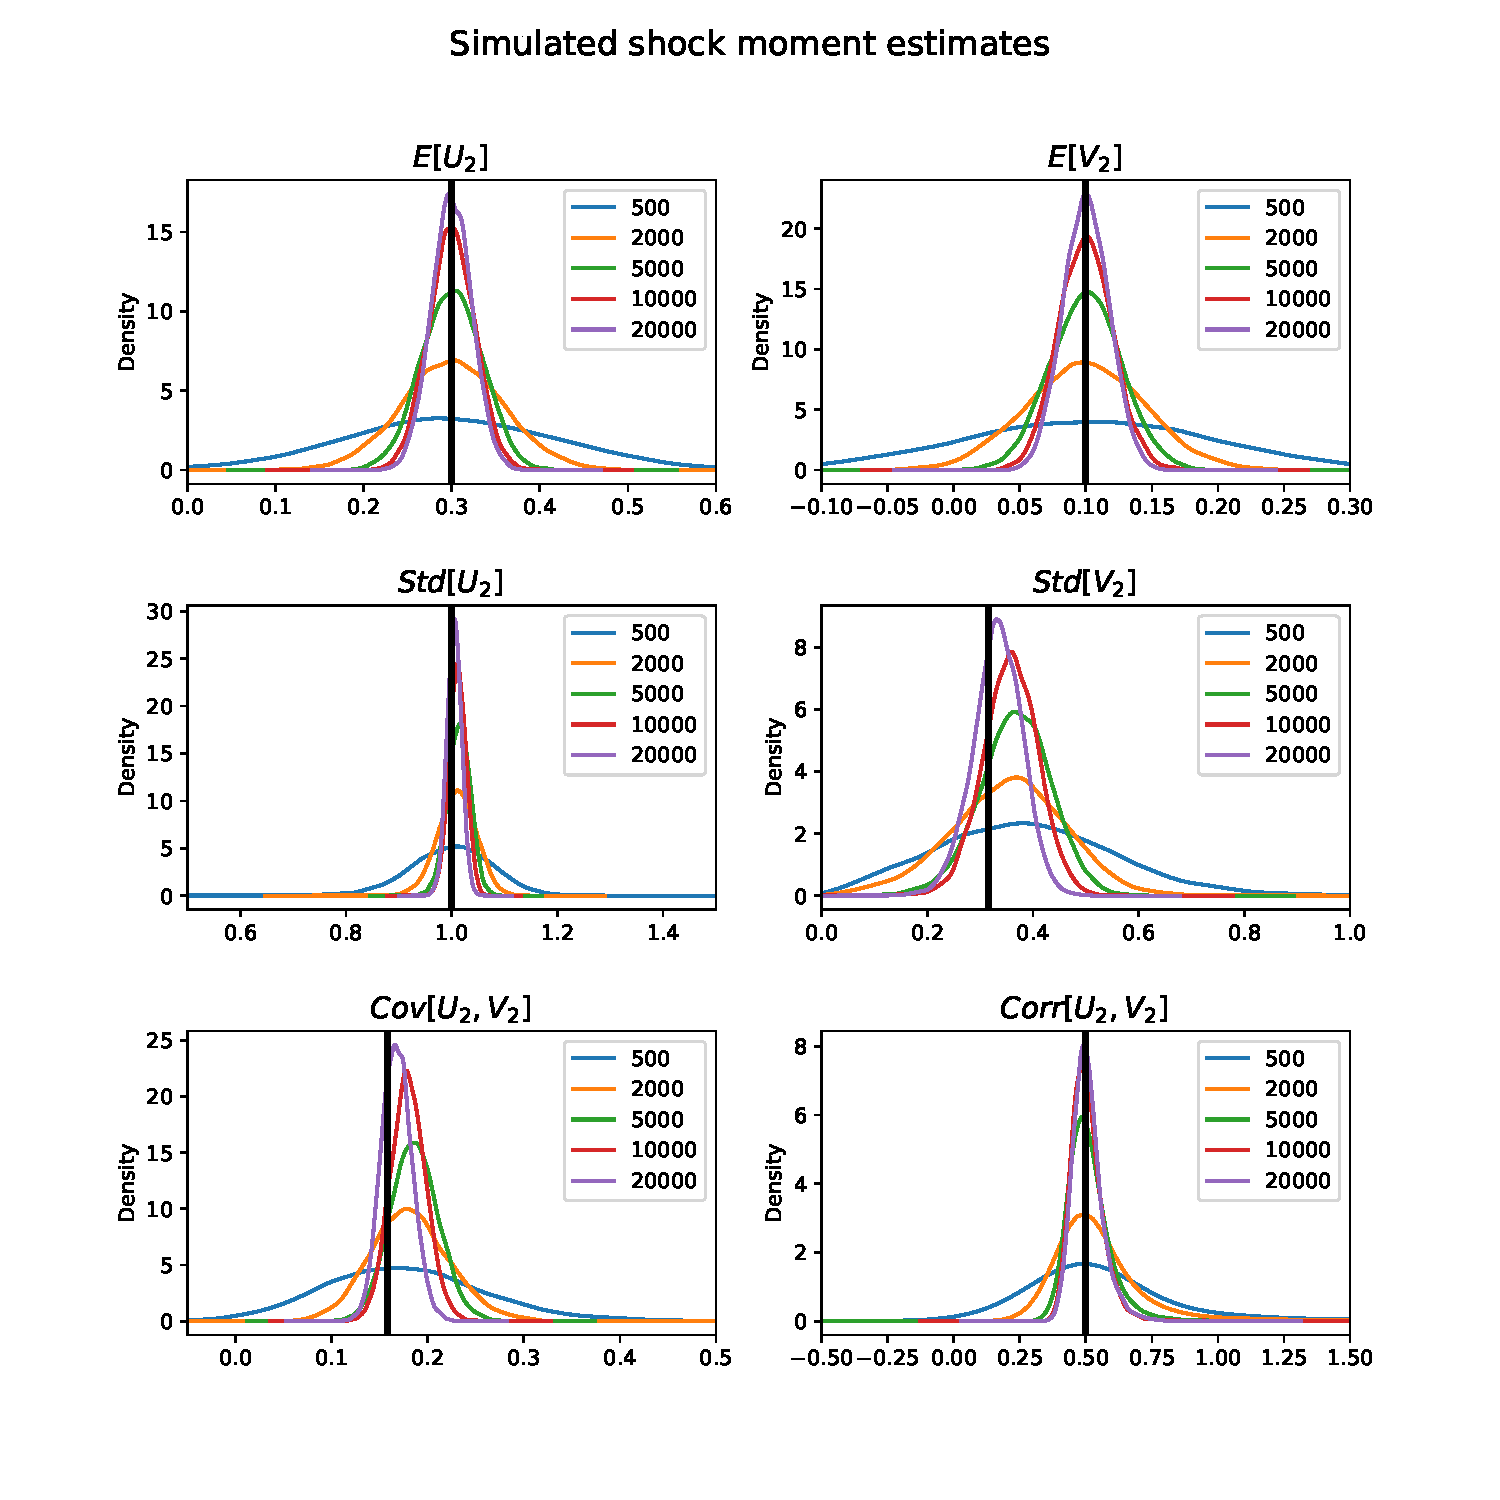
\includegraphics[height=0.8\textheight]{/Users/vitorhadad/Documents/kidney/matching/phd_thesis/chapter1/figures/simulation_shocks.pdf}
  \label{fig:simulation_shocks}
  \caption[Shock estimates in simulated data]{Shock estimates in simulated data}
\end{figure}

\begin{figure}
  \centering
  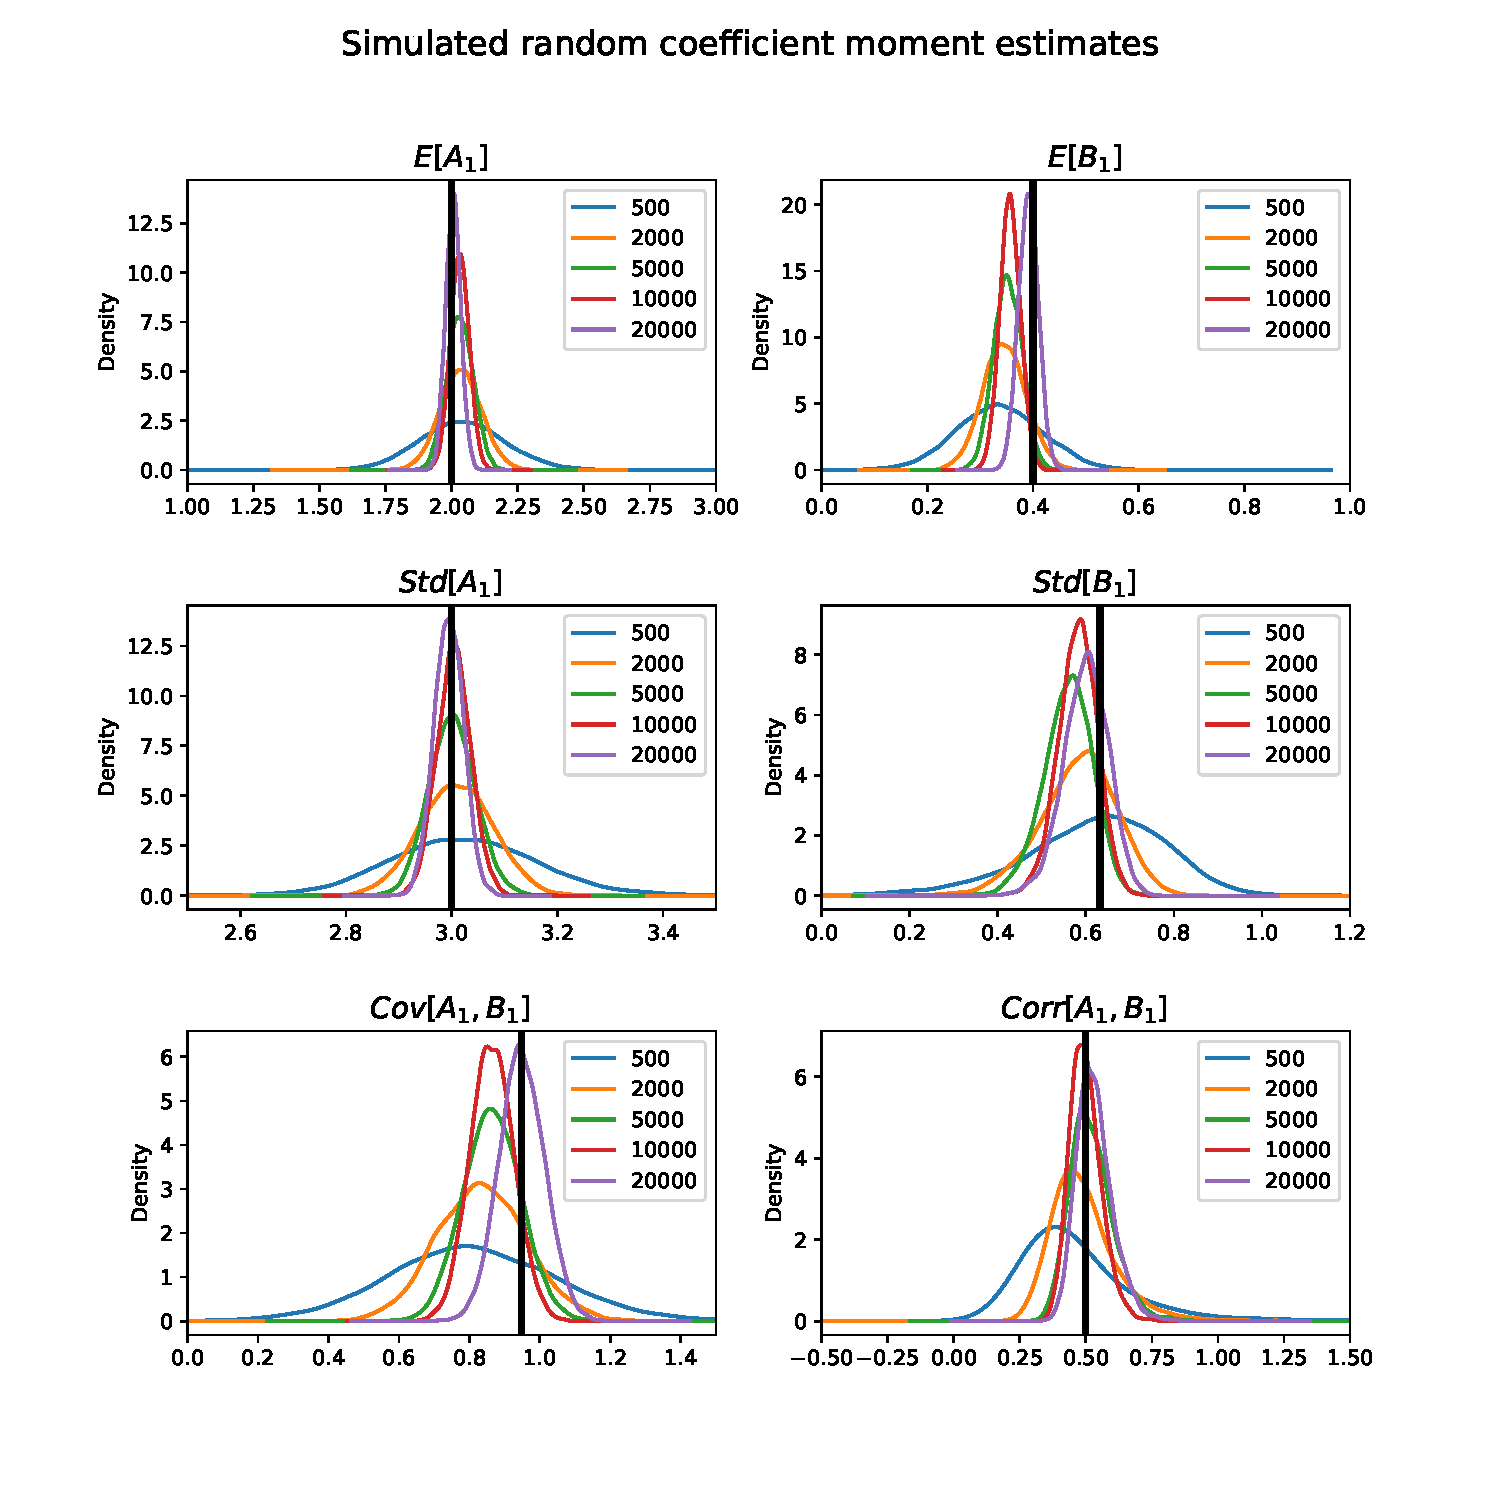
\includegraphics[height=0.8\textheight]{/Users/vitorhadad/Documents/kidney/matching/phd_thesis/chapter1/figures/simulation_random_coefficients.pdf}
  \label{fig:simulation_random_coefficients}
  \caption[Random coefficient estimates in simulated data]{Random coefficient estimates in simulated data}
\end{figure}

\begin{figure}
  \centering
  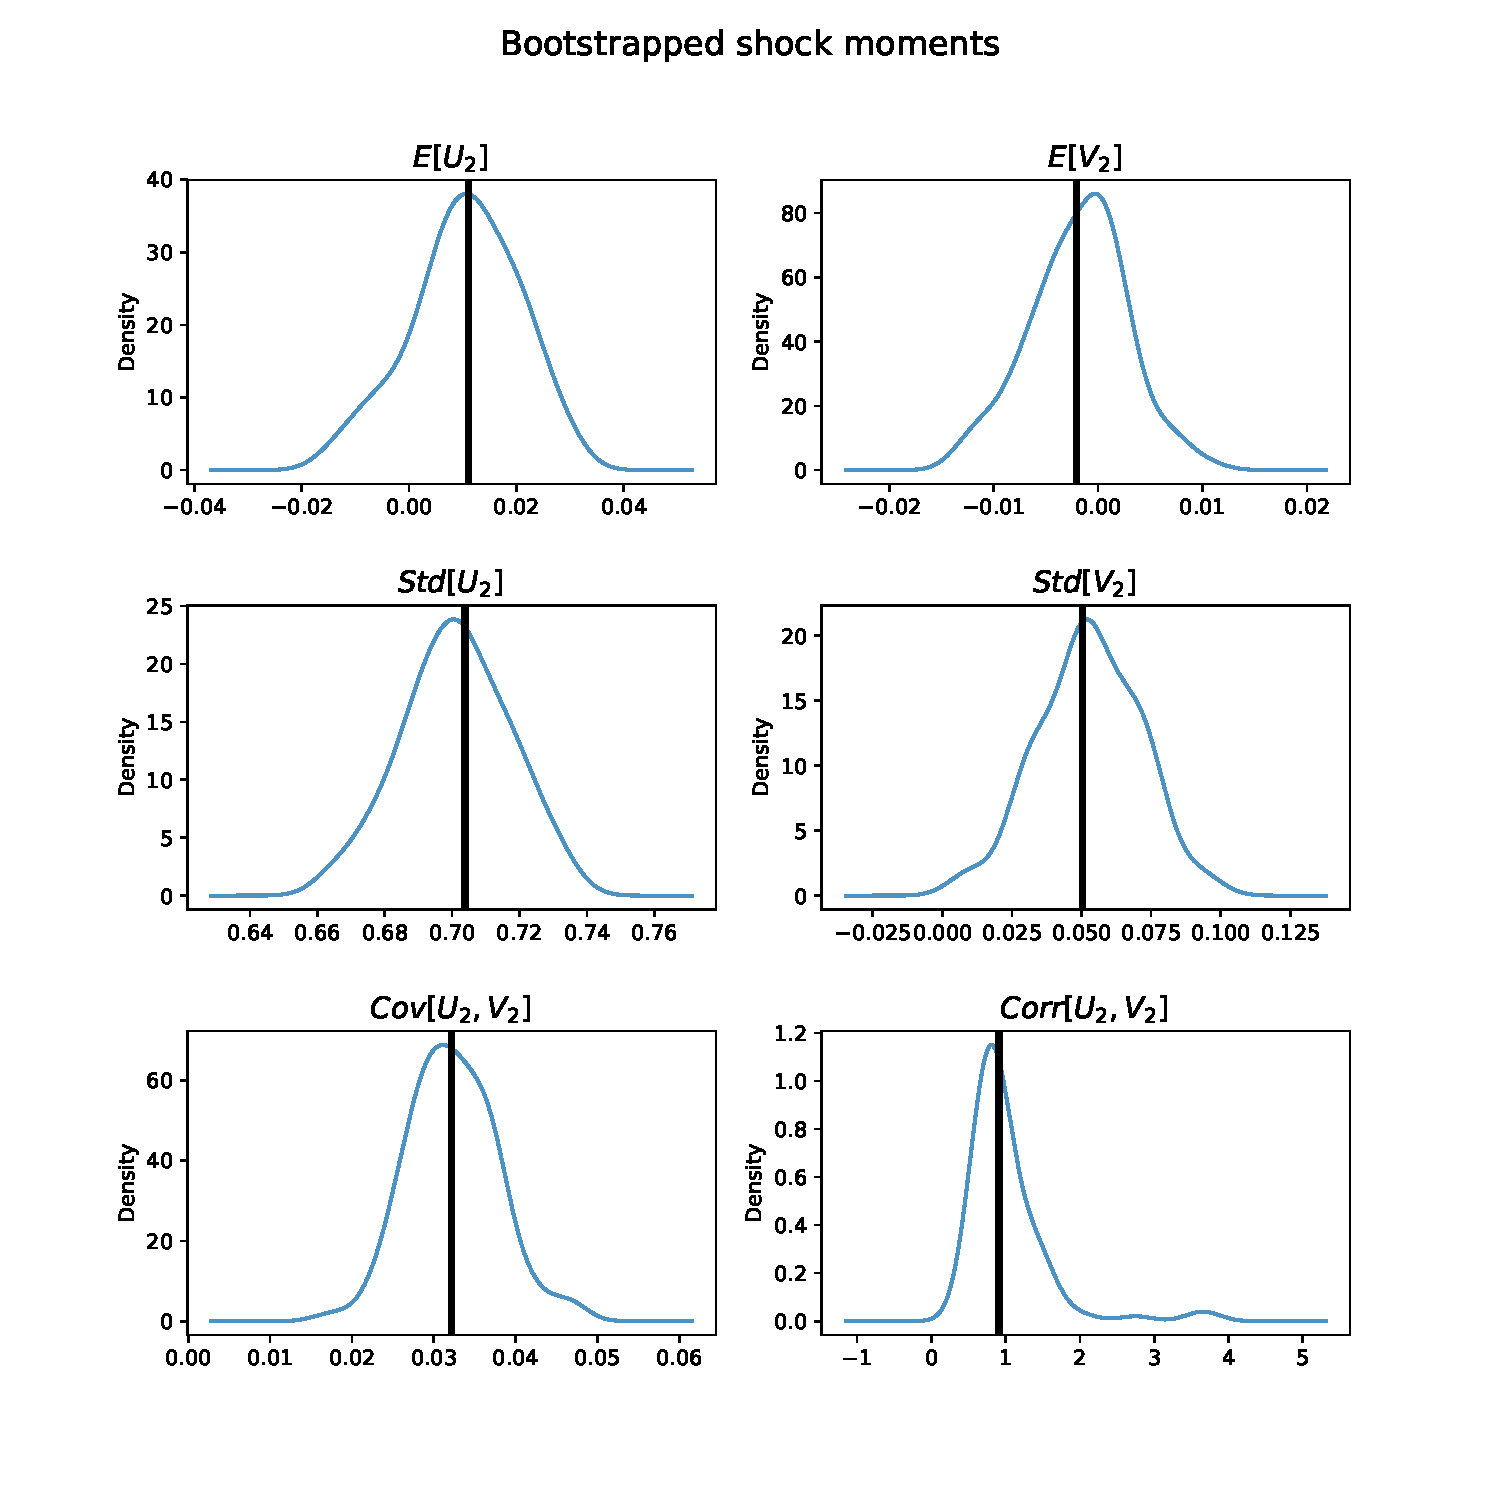
\includegraphics[height=0.8\textheight]{/Users/vitorhadad/Documents/kidney/matching/phd_thesis/chapter1/figures/shocks_empirical.pdf}
  \caption[Shock estimates using ASI data]{Shock estimates using ASI data}
\end{figure}


\begin{figure}
  \centering
  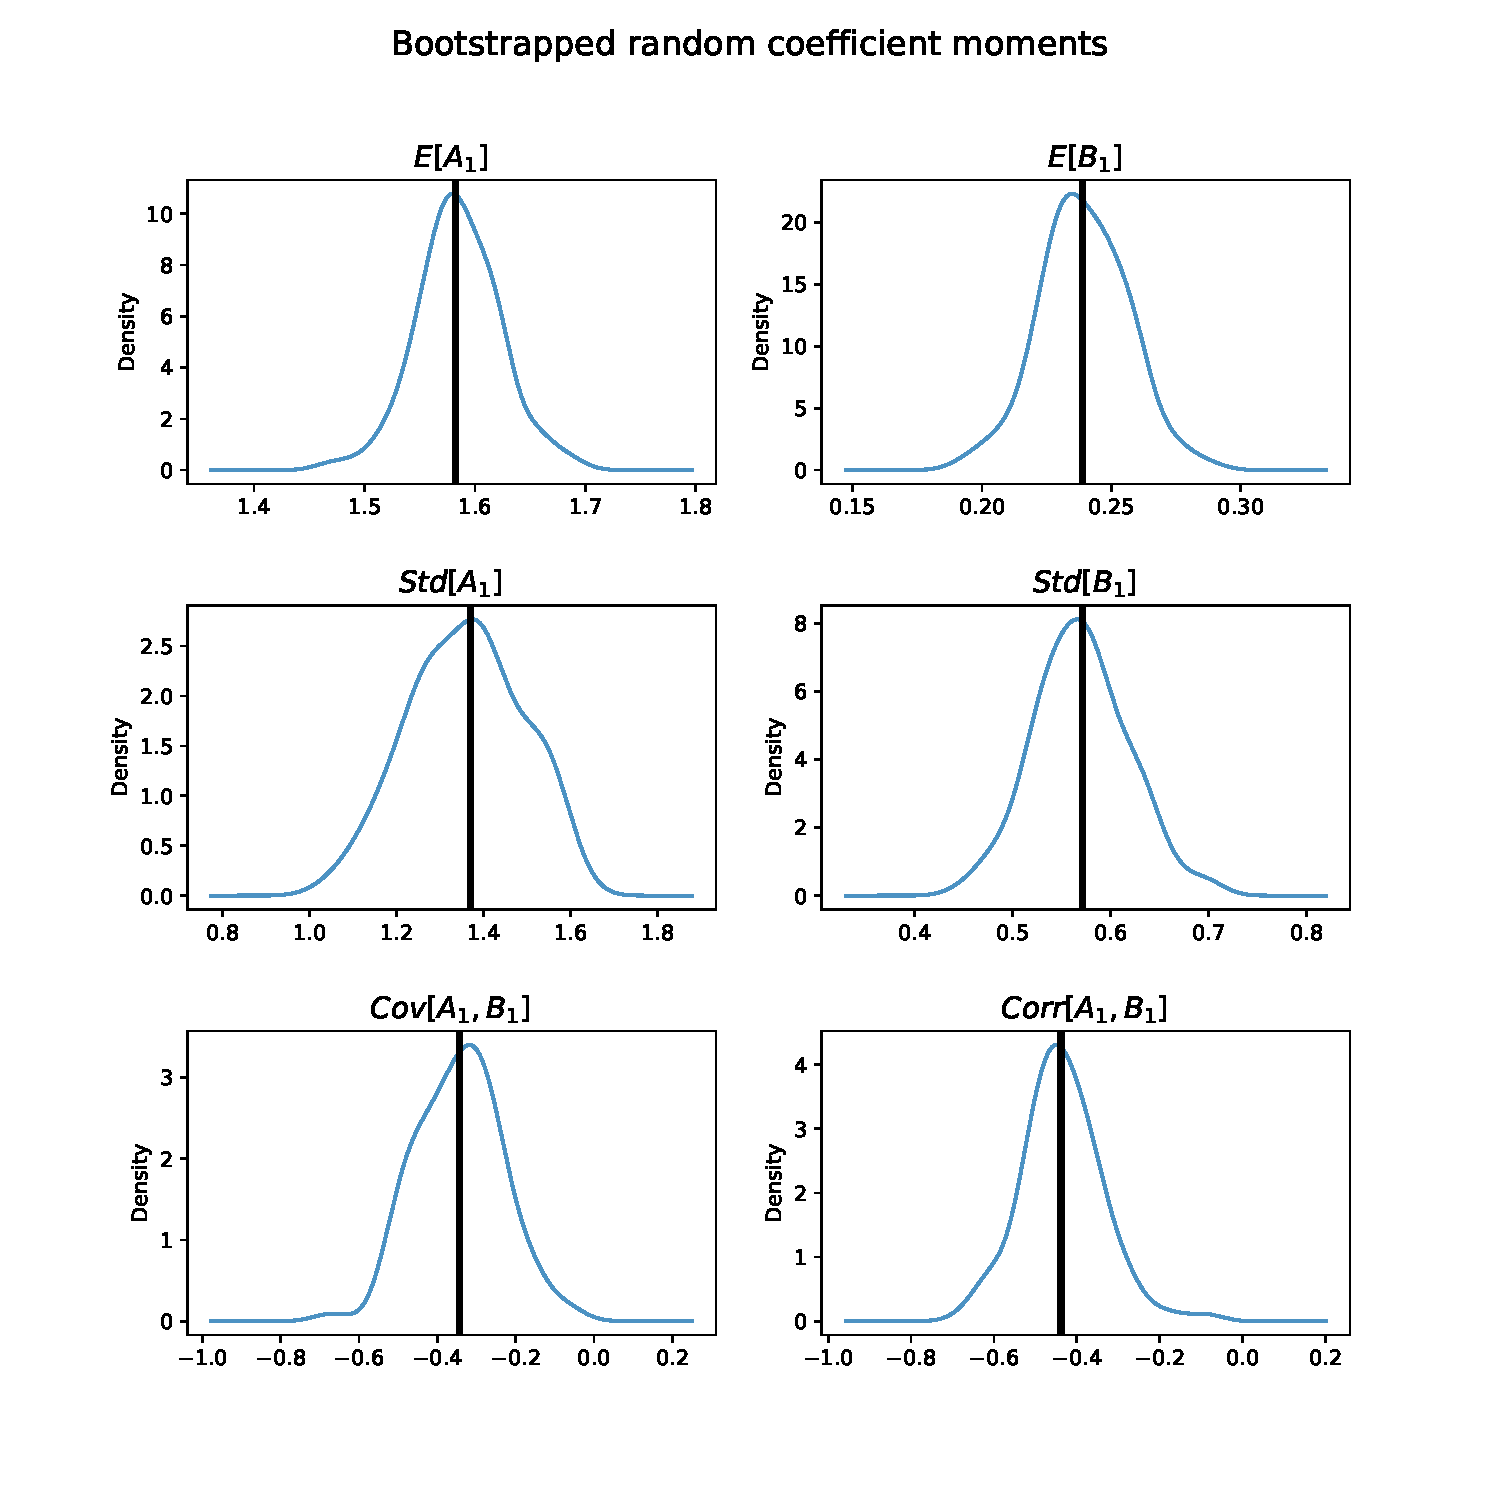
\includegraphics[height=0.8\textheight]{/Users/vitorhadad/Documents/kidney/matching/phd_thesis/chapter1/figures/rc1_empirical.pdf}
  \caption[Random coefficient estimates using ASI data (2008)]{Random coefficient estimates using ASI data (2008)}
\end{figure}

\begin{figure}
  \centering
  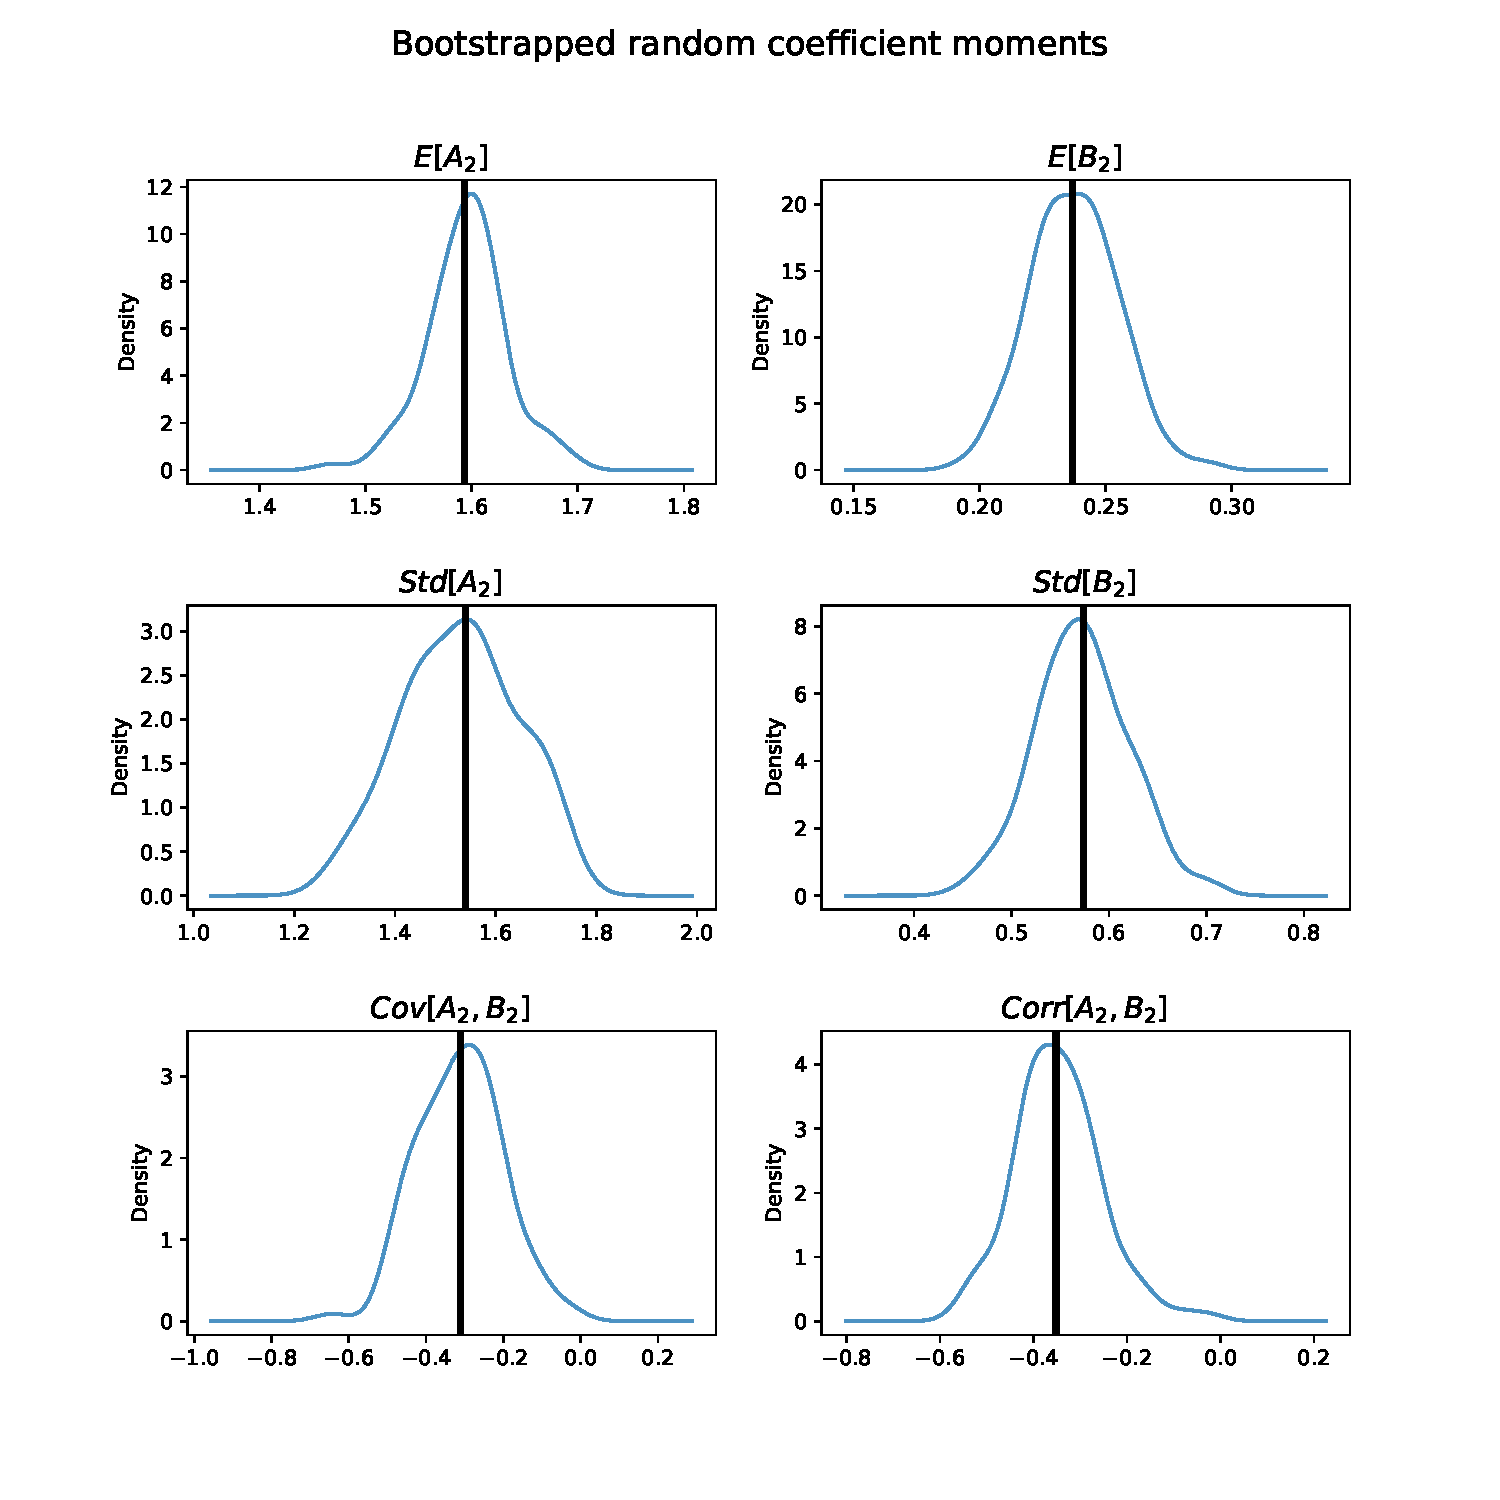
\includegraphics[height=0.8\textheight]{/Users/vitorhadad/Documents/kidney/matching/phd_thesis/chapter1/figures/rc2_empirical.pdf}
    \caption[Random coefficient estimates using ASI data (2009)]{Random coefficient estimates using ASI data (2009)}
\end{figure}





\clearpage


\section{Conclusion and future work}


What if T > 2? The approach generalizes but seems to become more complicated (as for example U2,V2 are correlated with X3,X4,...).
• It would be useful to see how strict the timing assumptions are (in standard linear panel models different timing assumptions can be dealt with by changing the set of instruments). For example: what if U2 independent of X1 but not of X2,X3,...?
• The authors’ setup could be used to learn about the firms’ ob- jectives, by estimating the determinants of input choice: Xit given
Ai,t−1, Bi,t−1, Xi,t−1, ....
• Looking ahead: nonlinear models? Example: CES.


% ------------
% APPENDIX
% ----------

\section{Appendix}

\subsection{Summary statistics} \label{sec:summary_statistics}



\begin{table}[H]
  \singlespacing
  \caption{ASI survey data: summary statistics}
  \begin{tabular}{lrrrrrrrr}
\toprule
{} &  $K_{2008}$ &  $M_{2008}$ &  $W_{2008}$ &  $S_{2008}$ &  $K_{2009}$ &  $M_{2009}$ &  $W_{2009}$ &  $S_{2009}$ \\
\midrule
mean &        16.8 &        17.9 &        15.6 &        18.4 &        16.8 &        17.9 &        15.6 &        18.4 \\
std  &        2.63 &        2.29 &        1.97 &        2.29 &        2.67 &        2.31 &        1.99 &        2.32 \\
min  &      -0.137 &         8.3 &        8.14 &         8.1 &      -0.207 &        7.96 &        7.85 &        5.83 \\
25\%  &        15.0 &        16.3 &        14.1 &        16.7 &        15.0 &        16.3 &        14.1 &        16.8 \\
50\%  &        17.0 &        18.1 &        15.8 &        18.6 &        17.0 &        18.2 &        15.8 &        18.7 \\
75\%  &        18.7 &        19.5 &        17.1 &        20.0 &        18.7 &        19.6 &        17.1 &        20.1 \\
max  &        26.3 &        27.1 &        23.3 &        27.4 &        26.2 &        27.2 &        23.2 &        27.4 \\
\bottomrule
\multicolumn{9}{p{.8\textwidth}}{{\scriptsize Variables are capital $K$, materials $M$, wages $W$ and sales value $S$. Variable units are 2005 rupees (in logs).}}
\end{tabular}

  \label{tab:summary_statistics_raw1}
\end{table}

\begin{table}[H]
  \singlespacing
  \caption{ASI survey data: correlations}
  \begin{tabular}{lrrrrrrrr}
\toprule
{} &  $K_{2008}$ &  $M_{2008}$ &  $W_{2008}$ &  $S_{2008}$ &  $K_{2009}$ &  $M_{2009}$ &  $W_{2009}$ &  $S_{2009}$ \\
\midrule
$K_{2008}$ &         1.0 &       0.825 &       0.808 &       0.827 &        0.98 &       0.822 &       0.812 &       0.829 \\
$M_{2008}$ &             &         1.0 &       0.843 &       0.976 &       0.823 &       0.963 &       0.834 &       0.948 \\
$W_{2008}$ &             &             &         1.0 &       0.861 &       0.802 &       0.817 &       0.971 &       0.839 \\
$Y_{2008}$ &             &             &             &         1.0 &       0.824 &       0.944 &       0.851 &        0.96 \\
$K_{2009}$ &             &             &             &        &         1.0 &       0.828 &       0.814 &       0.834 \\
$M_{2009}$ &             &             &             &        &             &         1.0 &       0.837 &       0.973 \\
$W_{2009}$ &             &             &             &        &              &            &         1.0 &       0.859 \\
$Y_{2009}$ &             &             &             &        &              &            &             &         1.0 \\
\bottomrule
\multicolumn{9}{p{.8\textwidth}}{{\scriptsize Correlations between capital $K$, materials $M$, wages $W$ and sales value $S$. Variable units are 2005 rupees (in logs).}}
\end{tabular}

  \label{tab:summary_statistics_raw2}
\end{table}


\begin{table}[H]
  \singlespacing
  \caption{Transformed variables: summary statistics}
  \begin{tabular}{lrrrr}
\toprule
{} &  $X_1$ &  $X_2$ &  $Y_1$ &  $Y_2$ \\
\midrule
mean &   1.05 &   1.09 &   1.83 &   1.82 \\
std  &   1.51 &   1.51 &   1.09 &   1.11 \\
min  &  -14.9 &  -15.9 &  -5.93 &  -7.12 \\
25\%  &  0.188 &  0.237 &   1.22 &   1.18 \\
50\%  &   1.15 &   1.18 &   1.83 &   1.82 \\
75\%  &   2.02 &   2.06 &   2.47 &   2.47 \\
max  &   7.96 &   7.96 &    6.5 &   9.75 \\
\bottomrule
\multicolumn{5}{l}{{\scriptsize $X = \log\left(\frac{K}{W}\right)$ and $Y=\log\left(\frac{S-M}{W}\right)$}}
\end{tabular}

  \label{tab:summary_statistics_processed1}
\end{table}

\begin{table}[H]
  \singlespacing
  \caption{Transformed variables: correlations}
  \begin{tabular}{lrrrr}
\toprule
{} &  $X_1$ &  $X_2$ &  $Y_1$ &  $Y_2$ \\
\midrule
$X_1$ &    1.0 &  0.911 &   0.43 &  0.401 \\
$X_2$ &    &    1.0 &  0.394 &  0.433 \\
$Y_1$ &    &         &    1.0 &  0.717 \\
$Y_2$ &    &        &        &    1.0 \\
\bottomrule
\multicolumn{5}{l}{{\scriptsize $X = \log\left(\frac{K}{W}\right)$ and $Y=\log\left(\frac{S-M}{W}\right)$}}
\end{tabular}

  \label{tab:summary_statistics_processed2}
\end{table}


\subsection{Simulation results}

Here we show how our estimates of shock and random coefficient moments change as we increase the number of observations. Throughout, we used the RMSE-minimizing parameters shown in table \ref{tab:best_parameters}. To produce the tables below, we generated 8000 datasets for each number different number of observations, produced the relevant estimates and computed the performance measures.

\subsubsection*{Shock moments}

\begin{table}[H]
  \singlespacing
  \caption{Performance measures for estimates of E[U_2]}
  \begin{tabular}{lrrrr}
\toprule
{} &    bias &  rel\_bias &  abs\_bias &   rmse \\
n     &         &           &           &        \\
\midrule
500   & -0.0013 &   -0.0043 &    0.0979 & 0.1230 \\
2000  &  0.0010 &    0.0032 &    0.0458 & 0.0576 \\
5000  &  0.0000 &    0.0001 &    0.0275 & 0.0342 \\
10000 & -0.0001 &   -0.0002 &    0.0208 & 0.0262 \\
20000 & -0.0001 &   -0.0003 &    0.0181 & 0.0227 \\
\bottomrule
\end{tabular}

\end{table}

\begin{table}[H]
  \singlespacing
  \caption{Performance measures for estimates of E[V_2]}
  \begin{tabular}{lrrrr}
\toprule
{} &    bias &  rel\_bias &  abs\_bias &   rmse \\
n     &         &           &           &        \\
\midrule
500   &  0.0002 &    0.0023 &    0.0776 & 0.0972 \\
2000  & -0.0001 &   -0.0014 &    0.0356 & 0.0446 \\
5000  &  0.0001 &    0.0006 &    0.0215 & 0.0270 \\
10000 & -0.0002 &   -0.0017 &    0.0163 & 0.0205 \\
20000 &  0.0003 &    0.0029 &    0.0139 & 0.0173 \\
\bottomrule
\end{tabular}

\end{table}

\begin{table}[H]
  \singlespacing
  \caption{Performance measures for estimates of Std[U_2]}
  \begin{tabular}{lrrrr}
\toprule
{} &    bias &  rel\_bias &  abs\_bias &   rmse \\
n     &         &           &           &        \\
\midrule
500   & -0.0021 &   -0.0021 &    0.0614 & 0.0780 \\
2000  &  0.0096 &    0.0096 &    0.0302 & 0.0379 \\
5000  &  0.0135 &    0.0135 &    0.0208 & 0.0256 \\
10000 &  0.0109 &    0.0109 &    0.0159 & 0.0197 \\
20000 &  0.0048 &    0.0048 &    0.0116 & 0.0145 \\
\bottomrule
\end{tabular}

\end{table}

\begin{table}[H]
  \singlespacing
  \caption{Performance measures for estimates of Std[B_2]}
  \begin{tabular}{lrrrr}
\toprule
{} &    bias &  rel\_bias &  abs\_bias &   rmse \\
n     &         &           &           &        \\
\midrule
500   & -0.0120 &   -0.0189 &    0.1242 & 0.1586 \\
2000  & -0.0515 &   -0.0815 &    0.0793 & 0.1034 \\
5000  & -0.0733 &   -0.1159 &    0.0771 & 0.0923 \\
10000 & -0.0512 &   -0.0810 &    0.0559 & 0.0677 \\
20000 & -0.0324 &   -0.0512 &    0.0474 & 0.0601 \\
\bottomrule
\end{tabular}

\end{table}

\begin{table}[H]
  \singlespacing
  \caption{Performance measures for estimates of Cov[U_2, V_2]}
  \begin{tabular}{lrrrr}
\toprule
{} &   bias &  rel\_bias &  abs\_bias &   rmse \\
n     &        &           &           &        \\
\midrule
500   & 0.0186 &    0.1175 &    0.0681 & 0.0873 \\
2000  & 0.0237 &    0.1499 &    0.0372 & 0.0473 \\
5000  & 0.0282 &    0.1786 &    0.0312 & 0.0376 \\
10000 & 0.0217 &    0.1375 &    0.0237 & 0.0285 \\
20000 & 0.0097 &    0.0614 &    0.0147 & 0.0186 \\
\bottomrule
\end{tabular}

\end{table}

\begin{table}[H]
  \singlespacing
  \caption{Performance measures for estimates of Corr[U_2, V_2]}
  \begin{tabular}{lrrrr}
\toprule
{} &   bias &  rel\_bias &  abs\_bias &   rmse \\
n     &        &           &           &        \\
\midrule
500   & 0.1198 &    0.2397 &    0.2586 & 0.6747 \\
2000  & 0.0736 &    0.1473 &    0.1387 & 0.3689 \\
5000  & 0.0145 &    0.0290 &    0.0613 & 0.1130 \\
10000 & 0.0050 &    0.0100 &    0.0456 & 0.0630 \\
20000 & 0.0077 &    0.0154 &    0.0437 & 0.0601 \\
\bottomrule
\end{tabular}

\end{table}


\subsection*{Random coefficient moments}

\begin{table}[H]
  \singlespacing
  \caption{Performance measures for estimates of E[A_1]}
  \begin{tabular}{lrrrr}
\toprule
{} &   bias &  rel\_bias &  abs\_bias &   rmse \\
n     &        &           &           &        \\
\midrule
500   & 0.0411 &    0.0205 &    0.1323 & 0.1669 \\
2000  & 0.0344 &    0.0172 &    0.0683 & 0.0856 \\
5000  & 0.0313 &    0.0157 &    0.0476 & 0.0591 \\
10000 & 0.0300 &    0.0150 &    0.0381 & 0.0467 \\
20000 & 0.0057 &    0.0029 &    0.0234 & 0.0293 \\
\bottomrule
\end{tabular}

\end{table}

\begin{table}[H]
  \singlespacing
  \caption{Performance measures for estimates of E[B_1]}
  \begin{tabular}{lrrrr}
\toprule
{} &    bias &  rel\_bias &  abs\_bias &   rmse \\
n     &         &           &           &        \\
\midrule
500   & -0.0637 &   -0.1593 &    0.0843 & 0.1035 \\
2000  & -0.0540 &   -0.1349 &    0.0578 & 0.0677 \\
5000  & -0.0479 &   -0.1197 &    0.0486 & 0.0547 \\
10000 & -0.0433 &   -0.1083 &    0.0435 & 0.0474 \\
20000 & -0.0085 &   -0.0212 &    0.0164 & 0.0205 \\
\bottomrule
\end{tabular}

\end{table}

\begin{table}[H]
  \singlespacing
  \caption{Performance measures for estimates of Std[A_1]}
  \begin{tabular}{lrrrr}
\toprule
{} &    bias &  rel\_bias &  abs\_bias &   rmse \\
n     &         &           &           &        \\
\midrule
500   &  0.0229 &    0.0076 &    0.1119 & 0.1411 \\
2000  &  0.0094 &    0.0031 &    0.0561 & 0.0702 \\
5000  &  0.0013 &    0.0004 &    0.0352 & 0.0443 \\
10000 &  0.0041 &    0.0014 &    0.0257 & 0.0323 \\
20000 & -0.0054 &   -0.0018 &    0.0226 & 0.0282 \\
\bottomrule
\end{tabular}

\end{table}
 
\begin{table}[H]
  \singlespacing
  \caption{Performance measures for estimates of Std[B_1]}
  \begin{tabular}{lrrrr}
\toprule
{} &    bias &  rel\_bias &  abs\_bias &   rmse \\
n     &         &           &           &        \\
\midrule
500   & -0.0120 &   -0.0189 &    0.1242 & 0.1586 \\
2000  & -0.0515 &   -0.0815 &    0.0793 & 0.1034 \\
5000  & -0.0733 &   -0.1159 &    0.0771 & 0.0923 \\
10000 & -0.0512 &   -0.0810 &    0.0559 & 0.0677 \\
20000 & -0.0324 &   -0.0512 &    0.0474 & 0.0601 \\
\bottomrule
\end{tabular}

\end{table}

\begin{table}[H]
  \singlespacing
  \caption{Performance measures for estimates of Cov[A_1, B_1]}
  \begin{tabular}{lrrrr}
\toprule
{} &    bias &  rel\_bias &  abs\_bias &   rmse \\
n     &         &           &           &        \\
\midrule
500   & -0.1401 &   -0.1477 &    0.2252 & 0.2790 \\
2000  & -0.1130 &   -0.1191 &    0.1396 & 0.1701 \\
5000  & -0.0840 &   -0.0885 &    0.0972 & 0.1174 \\
10000 & -0.0840 &   -0.0885 &    0.0892 & 0.1042 \\
20000 &  0.0006 &    0.0006 &    0.0513 & 0.0643 \\
\bottomrule
\end{tabular}

\end{table}
 
\begin{table}[H]
  \singlespacing
  \caption{Performance measures for estimates of Corr[A_1, B_1]}
  \begin{tabular}{lrrrr}
\toprule
{} &    bias &  rel\_bias &  abs\_bias &   rmse \\
n     &         &           &           &        \\
\midrule
500   & -0.0125 &   -0.0250 &    0.1913 & 0.3675 \\
2000  & -0.0042 &   -0.0085 &    0.0994 & 0.1554 \\
5000  &  0.0220 &    0.0440 &    0.0652 & 0.0862 \\
10000 & -0.0010 &   -0.0019 &    0.0476 & 0.0607 \\
20000 &  0.0333 &    0.0666 &    0.0576 & 0.0769 \\
\bottomrule
\end{tabular}

\end{table}

 
\subsection{Python module \texttt{FHHPS}}

In order to facilitate the adoption of the methods described in this paper by other researchers, I have developed the Python module \texttt{FHHPS}. Instructions for installations and usage can be found in the github repository\footnote{Url: https://github.com/halflearned/FHHPS}. Its API is inspired by the celebrated \texttt{scikit-learn} library\cite{sklearn_api}, and it should be familiar to statisticians and machine learning practitioners that use Python. The webpage linked above also contains one-line instructions for reproducing all of our figures and tables. 

\clearpage
\begin{landscape}
\begin{table}[H]
  \singlespacing
  \caption{Panel regressions}
  % Table created by stargazer v.5.2 by Marek Hlavac, Harvard University. E-mail: hlavac at fas.harvard.edu
% Date and time: Mon, Mar 26, 2018 - 22:31:53
% Table created by stargazer v.5.2 by Marek Hlavac, Harvard University. E-mail: hlavac at fas.harvard.edu
% Date and time: Mon, Mar 26, 2018 - 22:49:59
\begin{tabular}{@{\extracolsep{5pt}}lccccccccc} 
\\[-1.8ex]\hline 
\hline \\[-1.8ex] 
 & \multicolumn{9}{c}{$Y := \log(\frac{Output - Materials}{Wages})$ and $X := \frac{Capital}{Wages}$} \\ 
\cline{2-10} 
\\[-1.8ex] & \multicolumn{3}{c}{Y \textasciitilde X} & \multicolumn{2}{c}{Y \textasciitilde X + factor(panel\_group)} & \multicolumn{2}{c}{Y \textasciitilde X + factor(state)} & \multicolumn{2}{c}{Y \textasciitilde X + factor(nic1987)} \\ 
\\[-1.8ex] & (F) & (P) & (R) & (P) & (R) & (P) & (R) & (P) & (R)\\ 
\hline \\[-1.8ex] 
Intercept &  & 1.489$$ & 1.495$$ & 1.361$$ & 1.360$$ & 1.669$$ & 1.673$$ & 1.318$$ & 1.318$$ \\ 
 &  & (0.007) & (0.009) & (0.131) & (0.169) & (0.049) & (0.063) & (0.145) & (0.185) \\ 
 & & & & & & & & & \\ 
 X & 0.277$$ & 0.315$$ & 0.309$$ & 0.272$$ & 0.272$$ & 0.302$$ & 0.298$$ & 0.295$$ & 0.292$$ \\ 
  & (0.011) & (0.004) & (0.005) & (0.004) & (0.005) & (0.004) & (0.005) & (0.004) & (0.005) \\ 
  & & & & & & & & & \\ 
\hline \\[-1.8ex] 
R$^{2}$ & 0.045 & 0.186 & 0.135 & 0.271 & 0.196 & 0.205 & 0.148 & 0.276 & 0.202 \\ 
Adjusted R$^{2}$ & $-$0.909 & 0.186 & 0.135 & 0.262 & 0.186 & 0.204 & 0.147 & 0.275 & 0.201 \\ 
\hline 
\hline \\[-1.8ex] 
\textit{Note:}  & \multicolumn{9}{r}{F: Fixed effects, R: Random effects, P: Pooling. All coefficients significant with $p < 0.01$. N=13298, T=2.} \\ 
\end{tabular} 

  \label{tab:panel_lm_table}
\end{table}
\end{landscape}


 


